
\begin{center}
\textit{
	The results presented in this chapter are part of a first-author paper
	published in Monthly Notices of the Royal Astronomical Society, in which I
	led the majority of the analysis and writing.
}
\end{center}

\section{Introduction}
\label{ohno:sec:intro}
From a nucleosynthesis perspective, N is a unique element.
Along with C and He, it is one of only three elements lighter
than iron peak nuclei thought to owe a significant portion of its abundance
to asymptotic giant branch (AGB) stars~\citep[e.g.][]{Johnson2019}.
N is also the primary by-product of the CNO cycle, a cyclic nuclear reaction
that catalyses the conversion of H into He in stars more massive than the sun.
However, uncertainties surrounding the nucleosynthetic yields of N make it
difficult to model its abundances accurately.
Here we take an empirical approach to constrain N yields by using
state-of-the-art galactic chemical evolution (GCE) models to assess which
functional forms describing the yield can reproduce recent observational
data for gas phase abundances and trends in Milky Way disc stars found
by~\citet{Vincenzo2021b}.

\begin{figure*}
\centering
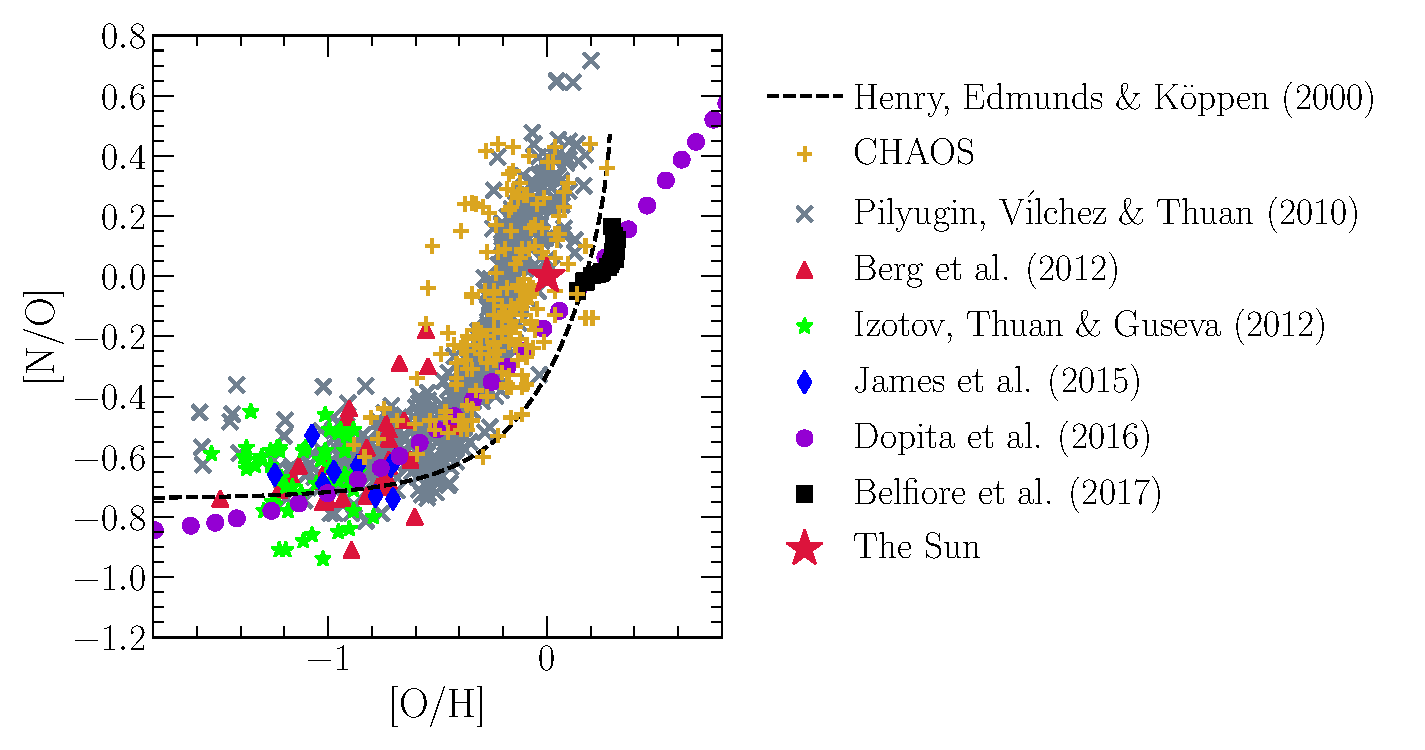
\includegraphics[scale = 0.65]{no_oh_observed.pdf}
\caption{
	The~\ohno~relation as observed in different galactic environments:
	HII regions from the first six CHAOS galaxies (golden +'s: NGC 3184, NGC
	628, NGC 5194, NGC 5457, M101, and NGC 2403;~\citealp{Berg2020,
	Skillman2020, Rogers2021}) and other nearby NGC spiral galaxies (grey X's;
	\citealp[][``ONS'' calibration]{Pilyugin2010}), HII regions in blue diffuse
	star forming dwarf galaxies (red triangles:~\citealp{Berg2012}; green stars:
	\citealp{Izotov2012}; blue diamonds:~\citealp{James2015}), in local stars
	and HII regions (purple circles:~\citealp{Dopita2016}), and in the MaNGA
	IFU survey (black squares:~\citealp{Belfiore2017}).
	The fit to~\no~as a function of~\oh~in Galactic and extragalactic HII
	regions by~\citet{Henry2000} is shown as a black dashed line.
	We omit all uncertainties for visual clarity.
	% {\color{red}
	All data have been normalized to the~\citet{Asplund2009} solar abundances,
	and the Sun is marked by a large red star.
	% }
}
\label{ohno:fig:no_oh_observed}
\end{figure*}

Observationally, N abundances in external galaxies are generally measured in
the gas phase and are used as a metallicity indicator because of their strong
correlation with O abundances.
In Fig.~\ref{ohno:fig:no_oh_observed}, we present a compilation of such measurements
along with data from the Milky Way:
\begin{enumerate}
	\item[\textbf{1.}] HII regions in the first six CHAOS\footnote{
		CHAOS: CHemical Abundances Of Spirals~\citep{Berg2015}
	} galaxies: NGC 3184, NGC 628, NGC 5194, NGC 5457, M101, and NGC 2403
	\citep{Berg2020, Skillman2020, Rogers2021}.

	\item[\textbf{2.}] HII regions in nearby NGC spirals
	\citep*[][``ONS'' calibration]{Pilyugin2010}.

	\item[\textbf{3.}] HII regions in blue, diffuse star forming dwarf galaxies
	(\citealp{Berg2012};~\citealp*{Izotov2012};~\citealp{James2015}).

	\item[\textbf{4.}] Local stars and HII regions~\citep{Dopita2016}.

	\item[\textbf{5.}] Galactic and extragalactic HII regions
	\citep*{Henry2000}.

	\item[\textbf{6.}] Star-forming regions in 550 nearby galaxies in the
	MaNGA IFU\footnote{
		MaNGA: Mapping Nearby Galaxies at Apache Point Observatory
		\citep{Bundy2015}.
		IFU: Integral Field Unit.
	} survey~\citep{Belfiore2017}.
\end{enumerate}
Despite intrinsic scatter and some systematic variation in how the abundances
are determined, this~\ohno\footnote{
	We follow standard notation where [X/Y]
	$\equiv \log_{10}(X/Y) - \log_{10}(X/Y)_\odot$.
} relation is found to be similar across a wide range of astrophysical
environments.
% mbox prevents this citation from getting split across pages and turning all
% of Fig. 1 into a giant hyperlink for Vincenzo & Kobayashi (2018).
Furthermore, recent arguments from both theoretical~\mbox{\citep{Vincenzo2018}}
and observational perspectives~\citep{HaydenPawson2022} suggest that this
relation is largely redshift-invariant.
Previous studies have interpreted this consistency as an indication that the
relation is nucleosynthetic in origin, reflective of a ``primary'' yield that
does not depend on a star's initial metal content and a ``secondary'' yield
that does (\citealp{VilaCostas1993};~\citealp*{vanZee1998};~\citealp{Henry1999,
PerezMontero2009};~\citealp*{Pilyugin2012};~\citealp{Andrews2013}).
Although we have highlighted star forming galaxies in
Fig.~\ref{ohno:fig:no_oh_observed}, N abundances are also easily measured in
massive ellipticals (see, e.g.,~\citealp{Schiavon2010},~\citealp{Conroy2013b},
and~\citealp*{Conroy2014} for observational references), allowing it to
potentially bridge the gap between the physical processes affecting galaxies of
different morphologies.
\par
The challenge in interpreting N abundances is that accurate nucleosynthetic
yields from various enrichment channels remain elusive.
Relative to other light elements, N synthesis is difficult to model because it
is sensitive to uncertain details of stellar evolution, such as internal
mixiing (see discussion in, e.g.,~\citealp{Andrews2017} and
in~\S~\ref{ohno:sec:yields:ccsne} below).
In this paper, we constrain N yields empirically by testing the performance of
various assumptions within the framework of GCE models.
To this end we make use of the multi-zone model for the Milky Way published by
\citet{Johnson2021}, which treats the Galaxy as a series of concentric rings,
describing each one as a conventional one-zone model of chemical evolution
(see discussion in~\S~\ref{ohno:sec:multizone}).
This approach has been employed in the past to compute abundances for many
Galactic regions simultaneously (\citealp{Matteucci1989, Wyse1989, Prantzos1995,
Schoenrich2009a};~\citealp*{Minchev2013, Minchev2014};~\citealp{Minchev2017};
\citealp*{Sharma2021}).
% {\color{red}
To ensure that our central conclusions are not affected by the model-dependent
nature of the GCE framework, we consider various parametrizations of the star
formation history (SFH), the initial mass function (IMF), and the absolute
scale of nucleosynthetic yields and Galactic winds.
% }%
Because of the apparent universality of the~\ohno~relation, our results using
the Milky Way as a case test should apply to other galaxies as well.
\par
At low metallicity, rotating massive stars play a key role in establishing the
observed N abundances (\citealp*{Chiappini2003, Chiappini2005};
\citealp{Chiappini2006};~\citealp*{Kobayashi2011};~\citealp{Prantzos2018};
\citealp*{Grisoni2021}).
Rotation plays a pivotal role in stellar evolution, inducing effects such as
shear mixing, meridional circulation, and horizontal turbulence~\citep{Zahn1992, 
Maeder1998, Lagarde2012}.
These effects carry internally produced C and O nuclei into the H-burning shell
where they can be processed into~\Nfourteen~via the CNO cycle~\citep{Heger2010,
Frischknecht2016, Andrews2017}.
Metal-poor stars spin faster and are more compact~\citep*{Maeder1999}, making
these effects stronger and consequently enhancing N yields~\citep*{Meynet2002a,
Meynet2002b, Meynet2006}.
We find similar results here comparing various theoretical models for massive
star nucleosynthesis (see discussion in~\S~\ref{ohno:sec:yields:ccsne}).
\par
% Recently,~\citet*{Grisoni2021} argued that rotating massive stars play a key
% role in establishing the N abundances seen in metal-poor stars in the Milky Way.
% Rotation has a considerable impact on the N yields of massive stars, because the
% internal mixing that it causes~\citep{Zahn1992, Maeder1998, Lagarde2012} brings
% internally produced C and O nuclei into the H-burning shell where they can be
% processed into~\Nfourteen~via the CNO cycle~\citep{Heger2010, Frischknecht2016,
% Andrews2017}.
% We find similar results here comparing various theoretical models for
% massive star nucleosynthesis (see discussion in~\S~\ref{ohno:sec:yields:ccsne}).
% \par
% Theoretical models for AGB star nucleosynthesis predict N yields to vary as a
% function of progenitor mass and metallicity~\citep{Cristallo2011, Cristallo2015,
% Karakas2010, Karakas2016, Karakas2018, Ventura2013, Ventura2014, Ventura2018,
% Ventura2020}.
In sufficiently massive AGB stars, the base of the convective envelope is hot
enough to activate proton capture reactions, allowing the CNO cycle to convert
C and O isotopes into~\Nfourteen: a process known as hot bottom burning (HBB).
AGB stars are also known to experience thermal pulses,
% {\color{red} \sout{pulsations} pulses}
and often these pulses
% {\color{red} \sout{pulsations} pulses}
are accompanied by a penetration of the convective enevelope into the
CO-rich core, which incorporates some of this material into the envelope
itself: a process known as third dredge-up (TDU).
When both processes are active, TDU adds new seed nuclei for HBB to turn
into~\Nfourteen, substantially increasing N yields.
We demonstrate in~\S\S~\ref{ohno:sec:yields:agb} and~\ref{ohno:sec:yields:imf_agb} that
various published theoretical models predict significantly discrepant N yields
for high mass AGB stars as a consequence of differences in TDU and
HBB.
The differences in these processes are in turn a consequence of the uncertain
% {\color{red} \sout{microphysical}}
assumptions built into stellar evolution models (e.g. mass
loss, opacity, convection and convective boundaries, nuclear reaction
networks).
In~\S~\ref{ohno:sec:results:yields}, we test the extent to which each of these
``off-the-shelf'' yield models are able to reproduce the~\ohno~relation in
GCE models.
\par
With a sample of 6,507 galaxies from the MaNGA IFU survey~\citep{Bundy2015},
\citet{Schaefer2020} demonstrate that the intrinsic scatter in
the~\ohno~relation at fixed galaxy mass is correlated with variations in the
local star formation efficiency (SFE).
In regions of slower star formation,~\no~tends to be slightly higher at
fixed~\oh~(see their fig. 4), which is expected from simple GCE models.
In classical ``closed-box models''~\citep[e.g.][]{Molla2006}, more AGB stars
enrich the interstellar medium (ISM) with N by the time a given~\oh~is reached,
whereas in ``open-box models'' with inflows and outflows like the ones we
present here, dilution by primordial gas accretion drives~\oh~down at fixed~\no.
However,~\citet{Schaefer2020} did not investigate stellar migration as a
potential source of additional scatter in the gas-phase~\ohno~relation.
In principle, there could be a deficit or surplus of N-producing AGB stars in a
given Galactic region at any time simply because the orbits are evolving,
driving additional scatter in the correlation.
The~\citet{Johnson2021} GCE model is an ideal tool with which to test this
hypothesis; the novel difference between theirs and previous models with
similar motivations is that it allows stellar populations to enrich
rings at different radii as they migrate.
Originally developed to study the abundances of O and Fe, this aspect of
Galactic evolution turned out to have an important impact on the delayed type
Ia supernova (SN Ia) enrichment of Fe, causing stochastic fluctuations in the
enrichment rates with time at fixed radius.
Here we use the same methodology to test for similar effects in the delayed AGB
star production of N, in turn assessing whether migration or variability in the
SFE dominate scatter in the~\ohno~relation.
\par
With stellar abundance data, we can test the N abundances predicted by our
model against observables unavailable for the gas phase, such as age and~\ofe.
Using data from the Apache Point Observatory Galaxy Evolution Experiment
(APOGEE;~\citealp{Majewski2017}) with asteroseismic mass measurements,
\citet{Vincenzo2021b} demonstrate that when stellar N abundances are corrected
for internal mixing processes, the correlations with stellar age and other
elemental abundances are affected.
Whether or not our GCE model is able to reproduce their data constitutes a
valuable test of our understanding of N nucleosynthesis and the history of N
enrichment in the Milky Way.
\citet{Vincenzo2021b} find good agreement between the APOGEE abundances and the
\citet{Dopita2016} data, which we find to be a good representation of external
galaxies as well; we therefore take the~\citet{Dopita2016} trend (the purple
points in Fig.~\ref{ohno:fig:no_oh_observed}) as our observational benchmark.
\par
In~\S~\ref{ohno:sec:yields}, we discuss our adopted yields of N from its dominant
nucleosynthetic sources.
We discuss the details of our multi-zone chemical evolution model
in~\S~\ref{ohno:sec:multizone}.
We describe the evolution of a fiducial model in~\S~\ref{ohno:sec:results:fiducial}.
In~\S~\ref{ohno:sec:results:yields}, we quantify the~\ohno~relation predicted by our
model with various ``off-the-shelf'' AGB star yield models taken from the
literature.
We investigate the relative importance of the delay-time distribution and the
metallicity-dependence of AGB star yields in~\S~\ref{ohno:sec:results:t_z_dep_comp}.
We compare our model predictions to stellar N abundances corrected for internal
mixing processes in~\S~\ref{ohno:sec:results:vincenzo_comp}.
We assess the sources of intrinsic scatter in the~\ohno~relation
in~\S~\ref{ohno:sec:results:schaefer_comp}.
We provide an analytic understanding of our key results
in~\S~\ref{ohno:sec:results:ohno_equilibrium} and summarize our conclusions
in~\S~\ref{ohno:sec:conclusions}.

